\section{Problem Statement}
\label{sec:formulation}

This section introduces the different components of the optimization problem to be solved. The formulation must accomplish the following criteria:
\begin{enumerate}
	\item Drive all agents from their starting position to their desired final positions.
	\item Respect a minimum pair-wise distance throughout the trajectory (collision constraint).
	\item The position and acceleration of the agents must be within specified boundaries.
\end{enumerate}

\subsection{The model}
The model used for each individual agent is a simple kinematic model of a unit mass in $\RR^3$. For simplicity, we use an abbreviated matrix representation as if the vectors were one-dimensional:
\begin{equation}
\label{eqn: model}
\begin{bmatrix}
p[k+1]\\
v[k+1]
\end{bmatrix} = \begin{bmatrix}
1 & h\\
0 & 1
\end{bmatrix} \begin{bmatrix}
p[k] \\
v[k]
\end{bmatrix} + \begin{bmatrix}
h^2/2 \\
h
\end{bmatrix}a[k]
\end{equation}
where vectors $p$, $v$ and $a$ are the discretized position, velocity and acceleration of the mass at time step $k = {0,1,\ldots,K-1}$, with $K$ being the length of the horizon and $h$ the time step duration in seconds. A compact representation is the following:
\begin{equation}
x[k+1] = Ax[k] + Bu[k] 
\end{equation}
where $x \in \RR^{6}$, $A \in \RR^{6\times 6} $, $B \in \RR^{6\times 3}$ and $u[k] \in \RR^{3}$. Expanding the model gives
\begin{equation}
\label{eqn:expand}
\begin{aligned}
x[1] &= Ax[0] + Bu[0]\\
x[2] &= A^2x[0] + ABu[0] + Bu[1]\\
&\vdots\\
x[K] &= A^{K}x[0] + A^{K-1}Bu[0] + \ldots + Bu[K-1]
\end{aligned}
\end{equation}
From Eqn.~(\ref{eqn:expand}), we can write the position sequence $P \in \RR^{3K}$ as an affine function of the input sequence $U \in \RR^{3K}$.
\begin{equation}
\label{eqn:model}
P = A_0X_0 + \Lambda U
\end{equation}
where $X_0 \in \RR^{6K}$ is the repeated sequence of initial states, and $\Lambda \in \RR^{3K \times 3K}$ is defined as
\begin{equation}
\Lambda = \begin{bmatrix}
\Psi B & 0 & \ldots & 0\\
\Psi AB & \Psi B & \ldots & 0 \\
\vdots & \ddots & \ddots & \vdots \\
\Psi A^{K-1}B & \Psi A^{K-2}B & \dots & \Psi B 
\end{bmatrix}
\end{equation}
with matrix $\Psi = \begin{bmatrix}
I_3 & 0
\end{bmatrix}$ selecting the first three rows of the matrix products (those corresponding the position states). 
Lastly, $A_0 \in \RR^{3K \times 6}$ is the propagation of the initial states
\begin{equation}
A_0 = \begin{bmatrix}
\Psi A & \Psi A^2 & \ldots & \Psi A^K
\end{bmatrix}^\top
\end{equation}

\subsection{Objective function}
The objective function has three main components: trajectory error, control effort and input variation. A similar formulation can be found in \cite{ru2017nonlinear}.

\subsubsection{Trajectory error penalty}
this term drives the agents to their goals. We want to minimize the error between the position at the final time step of the prediction horizon $p[K]$, and the desired final position $p_d$. The error term is given by
\begin{equation}
e = \norm {p[K]-p_d}_2
\end{equation}
which can be casted into a quadratic cost function of the input sequence, using Eqn.~(\ref{eqn:model}):
\begin{equation}
\label{eqn:error}
J_e = U^\top(\Lambda^{\top} \tilde{Q} \Lambda)U - 2(P_d^\top \tilde{Q} \Lambda -  A_0X_0 \tilde{Q} \Lambda)U
\end{equation}
Matrix $\tilde{Q} \in \RR^{3K \times 3K} $ is a positive semidefinite matrix that weights the error at each time step. Given that we want to enforce the trajectory to \textit{end} at the desired reference, then
\begin{equation}
\tilde{Q} = \begin{bmatrix}
0 & \ldots & 0 \\
\vdots & \ddots & \vdots \\
0 & \ldots & Q
\end{bmatrix}
\end{equation}
where $Q \in \RR^{3 \times 3}$ is chosen as a diagonal matrix that weights each coordinate of the position vector at the last time step of the horizon.

\subsubsection{Control effort penalty}
we also want to minimize the total control effort throughout the trajectory, through the following quadratic cost function:
\begin{equation}
\label{eqn:input}
J_u = U^\top \tilde{R} U 
\end{equation}
Similarly, $\tilde{R} \in \RR^{3K \times 3K} $ is positive semidefinite and weights the penalty on control effort
\begin{equation}
\tilde{R} = \begin{bmatrix}
R & 0& \ldots & 0 \\
0 & R & \ldots & 0 \\
\vdots & \ddots & \ddots & \vdots \\
0 & 0 & \ldots & R
\end{bmatrix}
\end{equation}
with $R \in \RR^{3 \times 3}$, a diagonal positive definite matrix.

\subsubsection{Input variation penalty}
this term is used to minimize variations of the acceleration, leading to smooth trajectories in position. Define the quadratic cost
\begin{equation}
\label{eqn:delta}
J_\delta = \sum_{k=0}^{K-1}\norm{u[k]-u[k-1]}^2
\end{equation}
To transform Eqn.~(\ref{eqn:delta}) into a quadratic form, define $\Delta \in \RR^{3K \times 3K}$
\begin{equation}
\Delta = \begin{bmatrix}
I_3 & 0 & 0 & \ldots & 0 & 0 \\
-I_3 & I_3 & 0 & \dots & 0 & 0 \\
0 & -I_3 & I_3 & \ldots & 0 & 0 \\
\vdots & \ddots & \ddots & \ddots & \vdots & \vdots\\
0& 0 & 0 & \ldots & -I_3 & I_3
\end{bmatrix}
\end{equation}
and define a vector $U_{-1} \in \RR^{3K}$ to include the term $u[-1]$ (which is a known constant at iteration $k$)

 \begin{figure*}
 	\centering
 	
 	\begin{subfloat}{
 		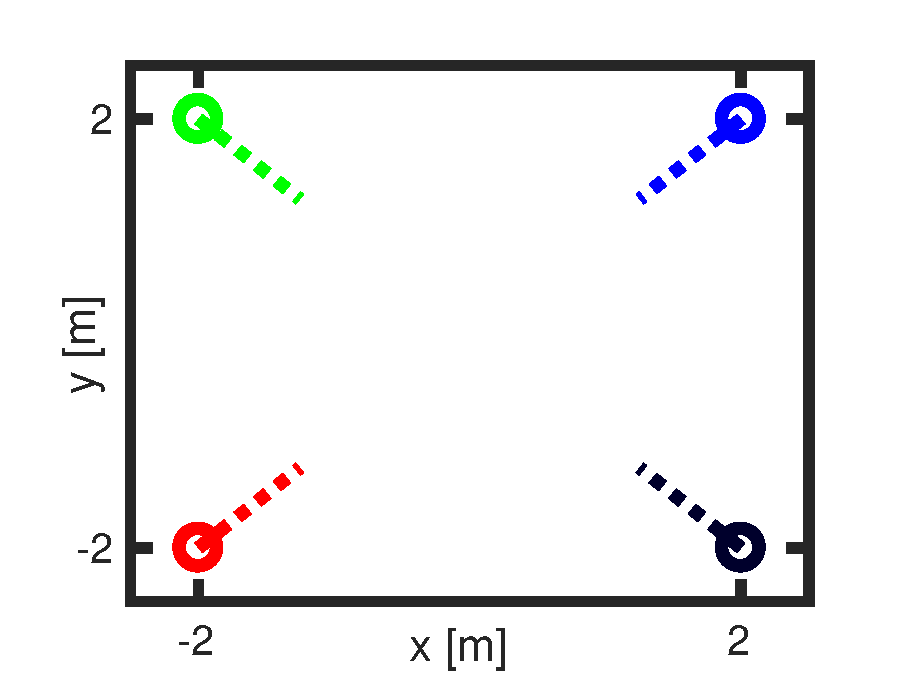
\includegraphics[width=0.26\textwidth]{figures/rail_a}}
 	\end{subfloat} \hspace{-5ex}
 	%
 	\begin{subfloat}{
 			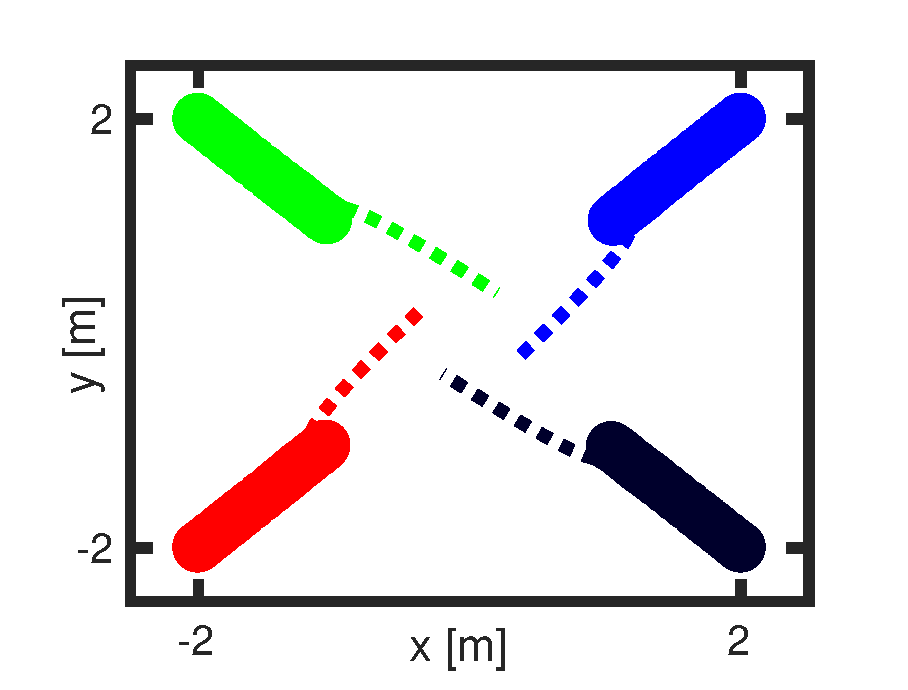
\includegraphics[width=0.26\textwidth]{figures/rail_b}}
 	\end{subfloat} \hspace{-5ex}
 	%
 	\begin{subfloat}{
 			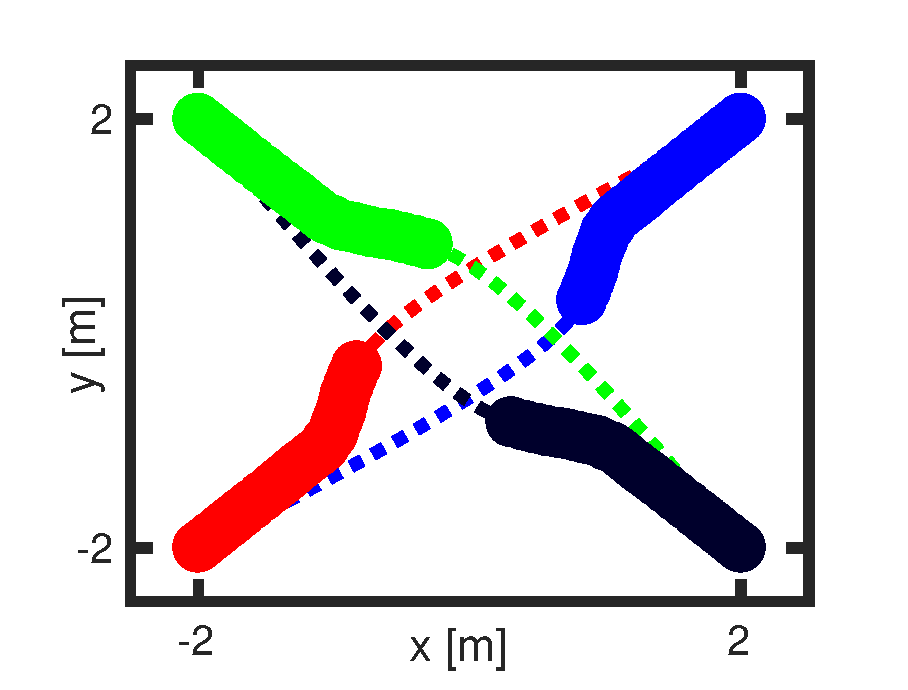
\includegraphics[width=0.26\textwidth]{figures/rail_c}}
 	\end{subfloat} \hspace{-5ex}
 	%
 	\begin{subfloat}{
 			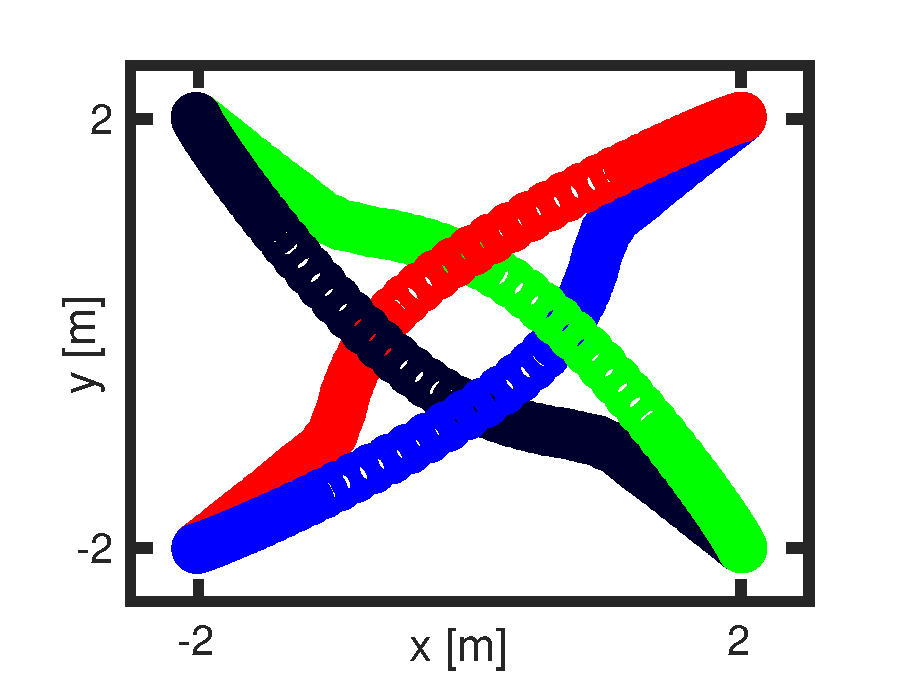
\includegraphics[width=0.26\textwidth]{figures/rail_d}}
 	\end{subfloat} 
 	\caption{4-vehicle position exchange scenario in 2D, solved using DMPC. The vehicles predict future collisions and slow down to safely circumvent the congested area. The result is a successful point-to-point transition, respecting all the constraints of the problem. }
 	\label{fig:four}
 \end{figure*}
\begin{equation}
U_{-1} = \begin{bmatrix}
u[-1] & 0 & \ldots & 0
\end{bmatrix}^\top
\end{equation}
Finally, we write Eqn.~(\ref{eqn:delta}) in quadratic form
\begin{equation}
\label{eqn:var}
J_\delta = U^\top (\Delta^\top \tilde{S} \Delta) U - 2(U_{-1}^\top \tilde{S} \Delta )U
\end{equation}	
where $\tilde{S} \in \RR^{3K \times 3K}$ is positive definite of the form

\begin{equation}
\tilde{S} = \begin{bmatrix}
S & 0& \ldots & 0 \\
0 & S & \ldots & 0 \\
\vdots & \ddots & \ddots & \vdots \\
0 & 0 & \ldots & S
\end{bmatrix}
\end{equation}
with $S \in \RR^{3 \times 3}$, a diagonal matrix.

The total cost function $\mathcal{J}$ is obtained by adding together Eqns.~(\ref{eqn:error},\ref{eqn:input},\ref{eqn:var})
\begin{equation}
\begin{aligned}
\mathcal{J}(U) &=  U^\top (\Lambda^{\top} \tilde{Q} \Lambda + \tilde{R} + \Delta^\top \tilde{S} \Delta) U \\
 & -2 (P_d^\top \tilde{Q} \Lambda -  A_0X_0 \tilde{Q} \Lambda + U_{-1}^\top \tilde{S} \Delta)U
\end{aligned}
\end{equation}	

\subsection{Collision avoidance}
To procure collision avoidance, each agent can access information of the most up-to-date prediction horizon of every other agent ($p_j$). When agent $i$ predicts a future collision at time step $k$ of the current prediction horizon, then it these collision constraints to its optimization problem
\begin{equation}
\label{eqn:coll}
\norm{p_i[k]-p_j[k]}_2 \geq r_{min} \quad \forall i,j = 1,2,\ldots,N \quad i \neq j
\end{equation}	

The non-convex constraint in Eqn.~(\ref{eqn:coll}) is linearized using a Taylor series expansion about the previous iterate $q$ of the predicted position horizon of agent $i$, $p_i^q$.
\begin{equation}
\label{eqn: taylor}
\norm{p^q_i[k] - p_j[k]}_2 + \frac{(p_i^q[k]-p_j[k])^\top}{\norm{p^q_i[k] - p_j[k]}_2}(p_i[k]-p_i^q[k]) \geq r_{min}
\end{equation}
The only variable in Eqn.~(\ref{eqn: taylor}) is $p_i[k]$, then it can can be expressed as
\begin{equation}
\label{eqn: bla}
(p_i^q[k]-p_j[k])^\top p_i[k] \geq \rho_j
\end{equation}
with
\begin{equation}
\begin{aligned}
\rho_j &= r_{min}\norm{p^q_i[k] - p_j[k]}_2 - \norm{p^q_i[k] - p_j[k]}_2^2 \\
& \hspace{1em}+ (p_i^q[k]-p_j[k])^\top p^q_i[k]
\end{aligned}
\end{equation}
Now, cast Eqn.~(\ref{eqn: bla}) into an affine function of the input $U$:
\begin{equation}
\Upsilon_j \Lambda U_i \geq \rho_j - \Upsilon_j A_0 x_i[0]
\end{equation}
where $\Upsilon_j \in \RR^{1 \times 3K}$ is defined as
\begin{equation}
\Upsilon_j = \begin{bmatrix}
0_{1\times 3k} & (p_i^q[k]-p_j[k])^\top & 0_{1 \times 3(K-1-k)}
\end{bmatrix}
\end{equation}
Finally, introduce $A_{coll,j} \in \RR^{1 \times 3K}$ and $b_{coll,j} \in \RR$
\begin{equation}
\label{eqn: coll}
A_{coll,j} = \Upsilon_j \Lambda ; \quad b_{coll,j} = \rho_j - \Upsilon_j A_0 x_i[0]
\end{equation}
The complete collision constraint matrices for agent $i$, $A_{coll} \in \RR^{(N-1) \times 3K}$ and $b_{coll} \in \RR^{(N-1)}$, can be obtained by stacking vertically the matrices in Eqn.~(\ref{eqn: coll}) for all the $N-1$ neighbours of agent $i$.


\subsection{Physical Limits}
The agents must remain within a specified volume and respecting acceleration limits, hence inequality constraints must be enforced both in the position and acceleration at each time step of the prediction horizon. Let $p_{min}, p_{max}, a_{min}, a_{max} \in \RR^3$ be the physical limits of the system. Define $P_{min}, P_{max}, U_{min}, U_{max} \in \RR^{3K}$:
\begin{equation}
\begin{aligned}
P_{min} = [p_{min} \ldots p_{min}]^\top; \quad  P_{max} = [p_{max} \ldots p_{max}]^\top \\
U_{min} = [a_{min} \ldots a_{min}]^\top; \quad  U_{max} = [a_{max} \ldots a_{max}]^\top
\end{aligned}
\end{equation}
Then, the physical limits constraints are formulated as
\begin{equation}
\begin{aligned}
P_{min} &\leq \Lambda U \leq P_{max} \\
U_{min} &\leq  U \leq U_{max}
\end{aligned}
\end{equation}

\subsection{Convex optimization problem}
The complete inequality constraints for agent $i$ are obtained by stacking vertically the collision avoidance and physical limits constraints. At each time step, agent $i$ solves the following convex optimization problem to update its prediction horizon
\begin{mini}|l|
	{U}{\mathcal{J}(U)}{}{}
	{\label{eqn:convex}}{}
	\addConstraint{A_{in}U}{\leq b_{in}}
\end{mini}
If collisions are predicted, then the problem would have $6K+N-1$ inequality constraints, otherwise the number is reduced to $6K$. The formulation in Eqn.~(\ref{eqn:convex}) results in a Quadratic Programming problem that can be computed efficiently. 
	
	